\section{Analysis of variance}
\frame{\sectionpage}

\begin{frame}[fragile]{Analysis of variance}

  \begin{itemize}
  \item Analysis of variance used with:
    \begin{itemize}
    \item counted/measured response
    \item categorical explanatory variable(s)
    \item that is, data divided into groups, and see if response significantly different among groups
    \item or, see whether knowing group membership helps to predict response.
    \end{itemize}
  \item Typically two stages:
    \begin{itemize}
    \item $F$-test to detect {\em any} differences among/due to groups
    \item if $F$-test significant, do {\em multiple comparisons} to see which groups significantly different from which.
    \item Need special multiple comparisons method because just doing (say) two-sample $t$-tests on each pair of groups gives too big a chance of finding ``significant'' differences by accident.
    \end{itemize}
  \end{itemize}
  
\end{frame}

\begin{frame}[fragile]{Example: Pain threshold and hair colour}
  
  \begin{itemize}
  \item Do people with different hair colour have different abilities
    to deal with pain?
  \item Men and women of various ages divided into 4 groups by hair
    colour: light and dark blond, light and dark brown.
  \item Each subject given a pain sensitivity test resulting in pain
    threshold score: higher score is higher pain tolerance.
  \item 19 subjects altogether.
  \end{itemize}

\end{frame}

\begin{frame}[fragile]{The data}
  
  In \texttt{hairpain.txt}:
  
  \begin{multicols}{2}
\begin{verbatim}
hair pain
lightblond 62
lightblond 60
lightblond 71
lightblond 55
lightblond 48
darkblond 63
darkblond 57
darkblond 52
darkblond 41
darkblond 43
lightbrown 42
lightbrown 50
lightbrown 41
lightbrown 37
darkbrown 32
darkbrown 39
darkbrown 51
darkbrown 30
darkbrown 35
\end{verbatim}
  \end{multicols}
  
\end{frame}

\begin{frame}[fragile]{Summarizing the groups}
  
  \begin{itemize}
    

  \item Read in data:
    
\begin{knitrout}
\definecolor{shadecolor}{rgb}{0.969, 0.969, 0.969}\color{fgcolor}\begin{kframe}
\begin{alltt}
\hlstd{hairpain}\hlkwb{=}\hlkwd{read.table}\hlstd{(}\hlstr{"hairpain.txt"}\hlstd{,}\hlkwc{header}\hlstd{=T)}
\end{alltt}
\end{kframe}
\end{knitrout}

\item then \texttt{aggregate}:
  
\begin{knitrout}
\definecolor{shadecolor}{rgb}{0.969, 0.969, 0.969}\color{fgcolor}\begin{kframe}
\begin{alltt}
\hlkwd{aggregate}\hlstd{(pain}\hlopt{~}\hlstd{hair,hairpain,mean)}
\end{alltt}
\begin{verbatim}
##         hair pain
## 1  darkblond 51.2
## 2  darkbrown 37.4
## 3 lightblond 59.2
## 4 lightbrown 42.5
\end{verbatim}
\end{kframe}
\end{knitrout}

\item Brown-haired people seem to have lower pain tolerance. 
  \end{itemize}
  
\end{frame}

\begin{frame}[fragile]{Or, better summary}
  
Use \texttt{dplyr}:

\begin{knitrout}
\definecolor{shadecolor}{rgb}{0.969, 0.969, 0.969}\color{fgcolor}\begin{kframe}
\begin{alltt}
\hlkwd{suppressMessages}\hlstd{(}\hlkwd{library}\hlstd{(dplyr))}
\hlstd{hairpain} \hlopt \hlkwd{group_by}\hlstd{(hair)} \hlopt
  \hlkwd{summarize}\hlstd{(} \hlkwc{n}\hlstd{=}\hlkwd{n}\hlstd{(),}
             \hlkwc{xbar}\hlstd{=}\hlkwd{mean}\hlstd{(pain),}
             \hlkwc{s}\hlstd{=}\hlkwd{sd}\hlstd{(pain))}
\end{alltt}
\begin{verbatim}
## # A tibble: 4 × 4
##         hair     n  xbar        s
##       <fctr> <int> <dbl>    <dbl>
## 1  darkblond     5  51.2 9.284396
## 2  darkbrown     5  37.4 8.324662
## 3 lightblond     5  59.2 8.526429
## 4 lightbrown     4  42.5 5.446712
\end{verbatim}
\end{kframe}
\end{knitrout}
  
\end{frame}

\begin{frame}[fragile]{Boxplot}
  
\begin{knitrout}
\definecolor{shadecolor}{rgb}{0.969, 0.969, 0.969}\color{fgcolor}\begin{kframe}
\begin{alltt}
\hlkwd{ggplot}\hlstd{(hairpain,}\hlkwd{aes}\hlstd{(}\hlkwc{x}\hlstd{=hair,}\hlkwc{y}\hlstd{=pain))}\hlopt{+}\hlkwd{geom_boxplot}\hlstd{()}
\end{alltt}
\end{kframe}
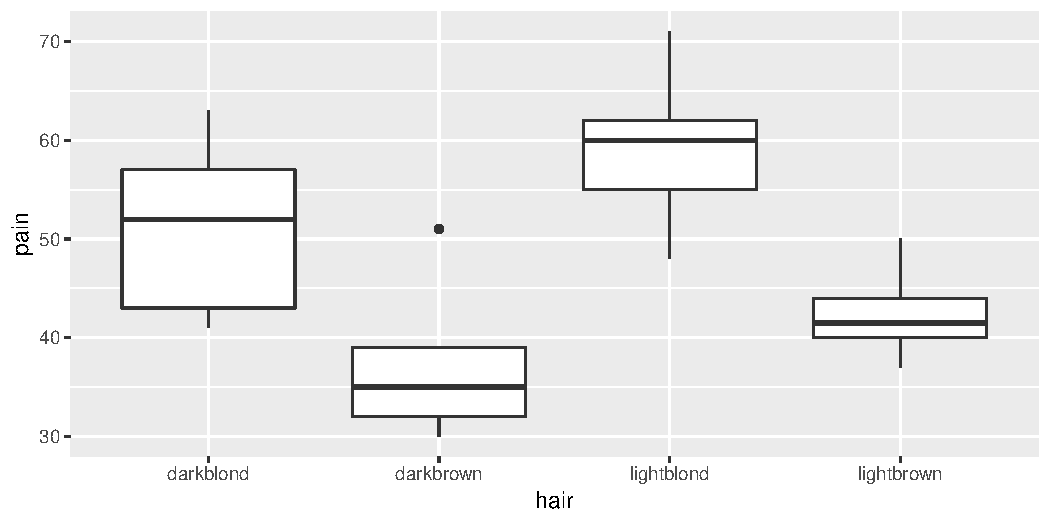
\includegraphics[width=\maxwidth]{figure/tartuffo-1} 

\end{knitrout}
  
\end{frame}

\begin{frame}[fragile]{Assumptions}
  
  \begin{itemize}
  \item Data should be:
    \begin{itemize}
    \item normally distributed within each group
    \item same spread for each group
    \end{itemize}

  \item \texttt{darkbrown} group has upper outlier (suggests not normal)
  \item \texttt{darkblond} group has smaller IQR than other groups.
  \item But, groups \emph{small}.
  \item Shrug shoulders and continue.
  \end{itemize}
  
\end{frame}

\begin{frame}[fragile]{Testing equality of SDs}
  
  
  \begin{itemize}
  \item   via \textbf{Levene's test}:
    {\small
\begin{knitrout}
\definecolor{shadecolor}{rgb}{0.969, 0.969, 0.969}\color{fgcolor}\begin{kframe}
\begin{alltt}
\hlstd{car}\hlopt{::}\hlkwd{leveneTest}\hlstd{(pain}\hlopt{~}\hlstd{hair,}\hlkwc{data}\hlstd{=hairpain)}
\end{alltt}
\begin{verbatim}
## Levene's Test for Homogeneity of Variance (center = median)
##       Df F value Pr(>F)
## group  3  0.3927   0.76
##       15
\end{verbatim}
\end{kframe}
\end{knitrout}
 }
\item No evidence (at all) of difference among group SDs.
\item Possibly because groups \emph{small}.
  \end{itemize}
  
\end{frame}

\begin{frame}[fragile]{Analysis of variance}
\begin{knitrout}
\definecolor{shadecolor}{rgb}{0.969, 0.969, 0.969}\color{fgcolor}\begin{kframe}
\begin{alltt}
\hlstd{hairpain.1}\hlkwb{=}\hlkwd{aov}\hlstd{(pain}\hlopt{~}\hlstd{hair,}\hlkwc{data}\hlstd{=hairpain)}
\hlkwd{summary}\hlstd{(hairpain.1)}
\end{alltt}
\begin{verbatim}
##             Df Sum Sq Mean Sq F value  Pr(>F)   
## hair         3   1361   453.6   6.791 0.00411 **
## Residuals   15   1002    66.8                   
## ---
## Signif. codes:  0 '***' 0.001 '**' 0.01 '*' 0.05 '.' 0.1 ' ' 1
\end{verbatim}
\end{kframe}
\end{knitrout}

\begin{itemize}
\item P-value small: the mean pain tolerances for the four groups are
  \emph{not} all the same.
\item Which groups differ from which, and how?
\end{itemize}
\end{frame}



\begin{frame}[fragile]{Multiple comparisons}

  \begin{itemize}
  \item Which groups differ from which? Multiple
    comparisons method. Lots.
  \item Problem: by comparing all the groups with each other, doing
    many tests, have large chance to (possibly incorrectly) reject
    $H_0:$ groups have equal means.
  \item 4 groups: 6 comparisons (1 vs 2, 1 vs 3, \ldots, 3 vs 4). 5 groups: 10
    comparisons. Thus 6 (or 10) chances to make mistake.
\item Get ``familywise error rate'' of 0.05 (whatever), no
matter how many comparisons you’re doing.
\item My favourite: Tukey, or ``honestly
  significant differences'': how far apart might largest, smallest
  group means be (if actually no differences). Group means more
  different: significantly different.
  \end{itemize}
\end{frame}

\begin{frame}[fragile]{Tukey}

  \begin{itemize}
  \item \texttt{TukeyHSD:}

{\footnotesize
 
\begin{knitrout}
\definecolor{shadecolor}{rgb}{0.969, 0.969, 0.969}\color{fgcolor}\begin{kframe}
\begin{alltt}
\hlkwd{TukeyHSD}\hlstd{(hairpain.1)}
\end{alltt}
\begin{verbatim}
##   Tukey multiple comparisons of means
##     95% family-wise confidence level
## 
## Fit: aov(formula = pain ~ hair, data = hairpain)
## 
## $hair
##                        diff        lwr        upr     p adj
## darkbrown-darkblond   -13.8 -28.696741  1.0967407 0.0740679
## lightblond-darkblond    8.0  -6.896741 22.8967407 0.4355768
## lightbrown-darkblond   -8.7 -24.500380  7.1003795 0.4147283
## lightblond-darkbrown   21.8   6.903259 36.6967407 0.0037079
## lightbrown-darkbrown    5.1 -10.700380 20.9003795 0.7893211
## lightbrown-lightblond -16.7 -32.500380 -0.8996205 0.0366467
\end{verbatim}
\end{kframe}
\end{knitrout}
}



  \end{itemize}



\end{frame}

\begin{frame}[fragile]{The old-fashioned way}
  
  \begin{itemize}
  \item List group means in order
  \item Draw lines connecting groups that are \emph{not} significantly
    different:
    
\begin{verbatim}
darkbrown lightbrown  darkblond lightblond
   37.4      42.5       51.2       59.2
   -------------------------
                        ---------------
\end{verbatim}

  \item \texttt{lightblond} significantly higher than everything
    except \texttt{darkblond} (at $\alpha=0.05$).
  \item \texttt{darkblond} in middle ground: not significantly less
    than \texttt{lightblond}, not significantly greater than
    \texttt{darkbrown} and \texttt{lightbrown}.
  \item More data might resolve this.
  \item Looks as if blond-haired people do have higher pain tolerance,
    but not completely clear.
  \end{itemize}
  
\end{frame}


\begin{frame}[fragile]{Some other multiple-comparison methods}

  \begin{itemize}
  \item P-values 0.005, 0.015, 0.03, 0.06 (4 tests all done at once)
Use $\alpha=0.05$.

\item Bonferroni: 
  \begin{itemize}
  \item 
Multiply all P-values by 4 (4 tests).
\item 
Reject only 1st null.
  \end{itemize}

\item Holm: 
  \begin{itemize}
  \item 
Times smallest P-value by 4: $0.005*4=0.020<0.05$, reject.
\item 
Times next smallest by 3: $0.015*3=0.045<0.05$, reject.
\item Times next smallest by 2: $0.03*2=0.06>0.05$, do not reject. Stop.
  \end{itemize}

\item False discovery rate:
  \begin{itemize}
  \item 
Times smallest P-value by 4: $0.005*4=0.02<0.05$: reject.
\item Times second smallest by $4/2$: $0.015*4/2=0.03<0.05$, reject.
\item Times third smallest by $4/3$: $0.03*4/3=0.04<0.05$, reject.
\item Times fourth smallest by $4/4$: 0.06*4/4=0.06>0.05, do not reject. Stop.
  \end{itemize}
  \end{itemize}
  
\end{frame}

\begin{frame}[fragile]{\texttt{pairwise.t.test}}

  \begin{multicols}{2}
{\tiny
\begin{knitrout}
\definecolor{shadecolor}{rgb}{0.969, 0.969, 0.969}\color{fgcolor}\begin{kframe}
\begin{alltt}
\hlkwd{attach}\hlstd{(hairpain)}
\hlkwd{pairwise.t.test}\hlstd{(pain,hair,}\hlkwc{p.adj}\hlstd{=}\hlstr{"none"}\hlstd{)}
\end{alltt}
\begin{verbatim}
## 
## 	Pairwise comparisons using t tests with pooled SD 
## 
## data:  pain and hair 
## 
##            darkblond darkbrown lightblond
## darkbrown  0.01748   -         -         
## lightblond 0.14251   0.00075   -         
## lightbrown 0.13337   0.36695   0.00817   
## 
## P value adjustment method: none
\end{verbatim}
\begin{alltt}
\hlkwd{pairwise.t.test}\hlstd{(pain,hair,}\hlkwc{p.adj}\hlstd{=}\hlstr{"holm"}\hlstd{)}
\end{alltt}
\begin{verbatim}
## 
## 	Pairwise comparisons using t tests with pooled SD 
## 
## data:  pain and hair 
## 
##            darkblond darkbrown lightblond
## darkbrown  0.0699    -         -         
## lightblond 0.4001    0.0045    -         
## lightbrown 0.4001    0.4001    0.0408    
## 
## P value adjustment method: holm
\end{verbatim}
\end{kframe}
\end{knitrout}

\begin{knitrout}
\definecolor{shadecolor}{rgb}{0.969, 0.969, 0.969}\color{fgcolor}\begin{kframe}
\begin{alltt}
\hlkwd{pairwise.t.test}\hlstd{(pain,hair,}\hlkwc{p.adj}\hlstd{=}\hlstr{"fdr"}\hlstd{)}
\end{alltt}
\begin{verbatim}
## 
## 	Pairwise comparisons using t tests with pooled SD 
## 
## data:  pain and hair 
## 
##            darkblond darkbrown lightblond
## darkbrown  0.0350    -         -         
## lightblond 0.1710    0.0045    -         
## lightbrown 0.1710    0.3670    0.0245    
## 
## P value adjustment method: fdr
\end{verbatim}
\begin{alltt}
\hlkwd{pairwise.t.test}\hlstd{(pain,hair,}\hlkwc{p.adj}\hlstd{=}\hlstr{"bon"}\hlstd{)}
\end{alltt}
\begin{verbatim}
## 
## 	Pairwise comparisons using t tests with pooled SD 
## 
## data:  pain and hair 
## 
##            darkblond darkbrown lightblond
## darkbrown  0.1049    -         -         
## lightblond 0.8550    0.0045    -         
## lightbrown 0.8002    1.0000    0.0490    
## 
## P value adjustment method: bonferroni
\end{verbatim}
\end{kframe}
\end{knitrout}
}
    
  \end{multicols}
  
\end{frame}

\begin{frame}[fragile]{Comments}
  
  \begin{itemize}
  \item P-values all adjusted upwards from ``none''.
  \item Required because 6 tests at once.
  \item Highest P-values for Bonferroni: most ``conservative''.
  \item Prefer Tukey or FDR or Holm.
  \item Tukey only applies to ANOVA, not to other cases of multiple
    testing. 
  \end{itemize}
  
\end{frame}

\begin{frame}[fragile]{Rats and vitamin B}
  
  \begin{itemize}
  \item What is the effect of dietary vitamin B on the kidney?
  \item A number of rats were randomized to receive either a
    B-supplemented diet or a regular diet.
  \item Desired to control for initial size of rats, so classified
    into size classes \texttt{lean} and \texttt{obese}.
  \item After 20 weeks, rats' kidneys weighed.
  \item Variables:
    \begin{itemize}
    \item Response: \texttt{kidneyweight} (grams).
    \item Explanatory: \texttt{diet}, \texttt{ratsize}.
    \end{itemize}
  \item Read in data:
    
\begin{knitrout}
\definecolor{shadecolor}{rgb}{0.969, 0.969, 0.969}\color{fgcolor}\begin{kframe}
\begin{alltt}
\hlstd{vitaminb}\hlkwb{=}\hlkwd{read.table}\hlstd{(}\hlstr{"vitaminb.txt"}\hlstd{,}\hlkwc{header}\hlstd{=T)}
\end{alltt}
\end{kframe}
\end{knitrout}
  \end{itemize}
  
\end{frame}

\begin{frame}[fragile]{What's going on?}
  
  \begin{itemize}
  \item Calculate group means:
    
\begin{knitrout}
\definecolor{shadecolor}{rgb}{0.969, 0.969, 0.969}\color{fgcolor}\begin{kframe}
\begin{alltt}
\hlstd{vitaminb} \hlopt \hlkwd{group_by}\hlstd{(ratsize,diet)} \hlopt
  \hlkwd{summarize}\hlstd{(}\hlkwc{mean}\hlstd{=}\hlkwd{mean}\hlstd{(kidneyweight))} \hlkwb{->} \hlstd{summary}
\hlstd{summary}
\end{alltt}
\begin{verbatim}
## Source: local data frame [4 x 3]
## Groups: ratsize [?]
## 
##   ratsize     diet     mean
##    <fctr>   <fctr>    <dbl>
## 1    lean  regular 1.641429
## 2    lean vitaminb 1.527143
## 3   obese  regular 2.642857
## 4   obese vitaminb 2.672857
\end{verbatim}
\end{kframe}
\end{knitrout}
\item Rat size: a large and consistent effect.
\item Diet: no effect (compare same rat size, different
  diet).
\item Effect of rat size \emph{same} for each diet: no interaction.
  \end{itemize}

\end{frame}

\begin{frame}[fragile]{ANOVA with interaction}
  
\begin{knitrout}
\definecolor{shadecolor}{rgb}{0.969, 0.969, 0.969}\color{fgcolor}\begin{kframe}
\begin{alltt}
\hlstd{vitaminb.1}\hlkwb{=}\hlkwd{aov}\hlstd{(kidneyweight}\hlopt{~}\hlstd{ratsize}\hlopt{*}\hlstd{diet,}\hlkwc{data}\hlstd{=vitaminb)}
\hlkwd{summary}\hlstd{(vitaminb.1)}
\end{alltt}
\begin{verbatim}
##              Df Sum Sq Mean Sq F value   Pr(>F)    
## ratsize       1  8.068   8.068 141.179 1.53e-11 ***
## diet          1  0.012   0.012   0.218    0.645    
## ratsize:diet  1  0.036   0.036   0.638    0.432    
## Residuals    24  1.372   0.057                     
## ---
## Signif. codes:  0 '***' 0.001 '**' 0.01 '*' 0.05 '.' 0.1 ' ' 1
\end{verbatim}
\end{kframe}
\end{knitrout}

Significance/nonsignificance as we expected. Note no significant
interaction (can be removed). 
  
\end{frame}

\begin{frame}[fragile]{Interaction plot}
  
  \begin{itemize}
  \item Plot mean of response variable against one of the explanatory, using
    other one as groups. Start from summary:
    
\begin{knitrout}
\definecolor{shadecolor}{rgb}{0.969, 0.969, 0.969}\color{fgcolor}\begin{kframe}
\begin{alltt}
\hlstd{g}\hlkwb{=}\hlkwd{ggplot}\hlstd{(summary,}\hlkwd{aes}\hlstd{(}\hlkwc{x}\hlstd{=ratsize,}\hlkwc{y}\hlstd{=mean,}
     \hlkwc{colour}\hlstd{=diet,}\hlkwc{group}\hlstd{=diet))}\hlopt{+}
  \hlkwd{geom_point}\hlstd{()}\hlopt{+}\hlkwd{geom_line}\hlstd{()}
\end{alltt}
\end{kframe}
\end{knitrout}

\item For this, have to give \emph{both} \texttt{group} and \texttt{colour}.
  \end{itemize}
  
\end{frame}

\begin{frame}[fragile]{The interaction plot}
\begin{knitrout}
\definecolor{shadecolor}{rgb}{0.969, 0.969, 0.969}\color{fgcolor}\begin{kframe}
\begin{alltt}
\hlstd{g}
\end{alltt}
\end{kframe}
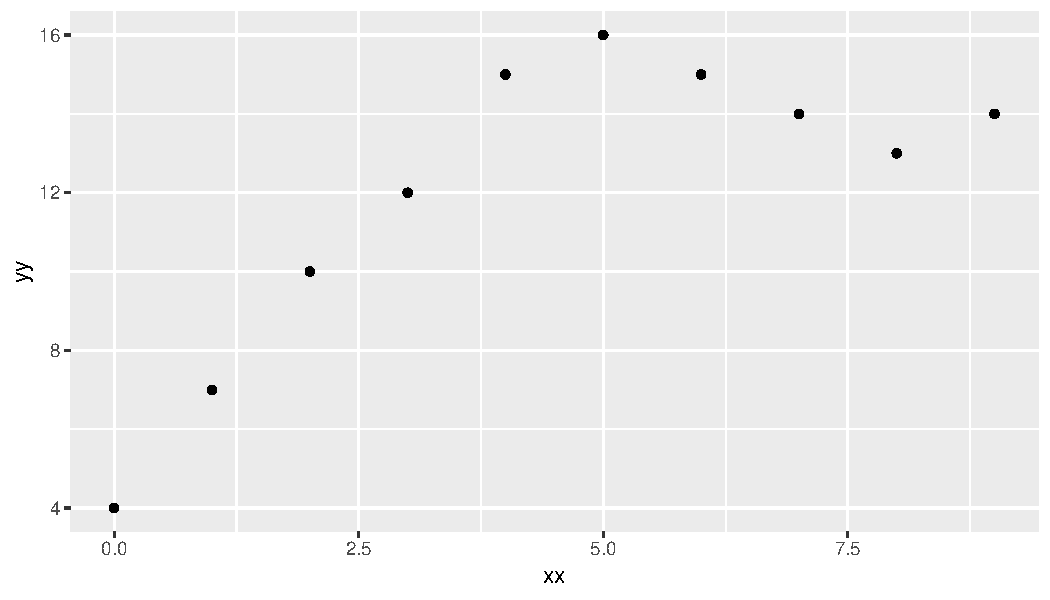
\includegraphics[width=\maxwidth]{figure/unnamed-chunk-14-1} 

\end{knitrout}

Lines basically parallel, indicating no interaction.
\end{frame}

\begin{frame}[fragile]{Take out interaction}
  
\begin{knitrout}
\definecolor{shadecolor}{rgb}{0.969, 0.969, 0.969}\color{fgcolor}\begin{kframe}
\begin{alltt}
\hlstd{vitaminb.2}\hlkwb{=}\hlkwd{aov}\hlstd{(kidneyweight}\hlopt{~}\hlstd{ratsize}\hlopt{+}\hlstd{diet,}\hlkwc{data}\hlstd{=vitaminb)}
\hlkwd{summary}\hlstd{(vitaminb.2)}
\end{alltt}
\begin{verbatim}
##             Df Sum Sq Mean Sq F value   Pr(>F)    
## ratsize      1  8.068   8.068 143.256 7.59e-12 ***
## diet         1  0.012   0.012   0.221    0.643    
## Residuals   25  1.408   0.056                     
## ---
## Signif. codes:  0 '***' 0.001 '**' 0.01 '*' 0.05 '.' 0.1 ' ' 1
\end{verbatim}
\end{kframe}
\end{knitrout}

\begin{itemize}
\item No Tukey for \texttt{diet}: not significant.
\item No Tukey for \texttt{ratsize}: only two sizes, and already know
  that obese rats have larger kidneys than lean ones.
\item Bottom line: diet has no effect on kidney size once you control
  for size of rat.
\end{itemize}
  
\end{frame}



\begin{frame}[fragile]{The auto noise data}
  
  In 1973, the President of Texaco cited an automobile filter
  developed by Associated Octel Company as effective in reducing
  pollution. However, questions had been raised about the effects of
  filter silencing. He referred to the data included in the report
  (and below) as evidence
  that the silencing properties of the Octel filter were at least
  equal to those of standard silencers. 
 
\begin{knitrout}
\definecolor{shadecolor}{rgb}{0.969, 0.969, 0.969}\color{fgcolor}\begin{kframe}
\begin{alltt}
\hlstd{autonoise}\hlkwb{=}\hlkwd{read.table}\hlstd{(}\hlstr{"autonoise.txt"}\hlstd{,}\hlkwc{header}\hlstd{=T)}
\hlkwd{str}\hlstd{(autonoise)}
\end{alltt}
\begin{verbatim}
## 'data.frame':	36 obs. of  4 variables:
##  $ noise: int  840 770 820 775 825 840 845 825 815 845 ...
##  $ size : Factor w/ 3 levels "L","M","S": 2 1 2 1 2 2 2 2 2 2 ...
##  $ type : Factor w/ 2 levels "Octel","Std": 2 1 1 1 1 2 2 1 1 2 ...
##  $ side : Factor w/ 2 levels "L","R": 2 1 2 2 1 2 1 1 1 2 ...
\end{verbatim}
\end{kframe}
\end{knitrout}
  
\end{frame}

\begin{frame}[fragile]{Making boxplot}
  
  \begin{itemize}
  \item Make a boxplot, but have combinations of filter type and
    engine size.
  \item Make a column that is the two of them glued together, and then
    use as $x$ for boxplot:
    
\begin{knitrout}
\definecolor{shadecolor}{rgb}{0.969, 0.969, 0.969}\color{fgcolor}\begin{kframe}
\begin{alltt}
\hlstd{autonoise} \hlopt \hlkwd{unite}\hlstd{(sizetype,}\hlkwd{c}\hlstd{(size,type))} \hlopt \hlkwd{head}\hlstd{()}
\end{alltt}
\begin{verbatim}
##   noise sizetype side
## 1   840    M_Std    R
## 2   770  L_Octel    L
## 3   820  M_Octel    R
## 4   775  L_Octel    R
## 5   825  M_Octel    L
## 6   840    M_Std    R
\end{verbatim}
\end{kframe}
\end{knitrout}

\item Pipe also plays with \texttt{ggplot}, thus:
  
\begin{knitrout}
\definecolor{shadecolor}{rgb}{0.969, 0.969, 0.969}\color{fgcolor}\begin{kframe}
\begin{alltt}
\hlstd{autonoise} \hlopt \hlkwd{unite}\hlstd{(sizetype,}\hlkwd{c}\hlstd{(size,type))} \hlopt
  \hlkwd{ggplot}\hlstd{(}\hlkwd{aes}\hlstd{(}\hlkwc{x}\hlstd{=sizetype,}\hlkwc{y}\hlstd{=noise))}\hlopt{+}\hlkwd{geom_boxplot}\hlstd{()} \hlkwb{->} \hlstd{g}
\end{alltt}
\end{kframe}
\end{knitrout}
  \end{itemize}
  
  
\end{frame}

\begin{frame}[fragile]{The boxplot}
\begin{knitrout}
\definecolor{shadecolor}{rgb}{0.969, 0.969, 0.969}\color{fgcolor}\begin{kframe}
\begin{alltt}
\hlstd{g}
\end{alltt}
\end{kframe}
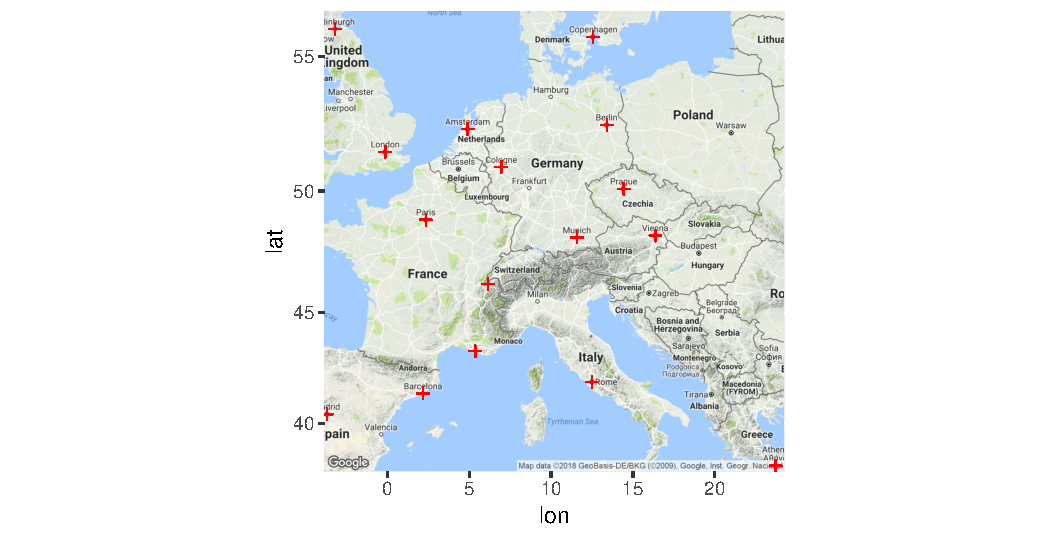
\includegraphics[width=\maxwidth]{figure/unnamed-chunk-19-1} 

\end{knitrout}

Difference in engine noise between Octel and standard is larger for
medium engine size than for large or small.
\end{frame}


\begin{frame}[fragile]{ANOVA}
  
\begin{knitrout}
\definecolor{shadecolor}{rgb}{0.969, 0.969, 0.969}\color{fgcolor}\begin{kframe}
\begin{alltt}
\hlstd{autonoise.1}\hlkwb{=}\hlkwd{aov}\hlstd{(noise}\hlopt{~}\hlstd{size}\hlopt{*}\hlstd{type,}\hlkwc{data}\hlstd{=autonoise)}
\hlkwd{summary}\hlstd{(autonoise.1)}
\end{alltt}
\begin{verbatim}
##             Df Sum Sq Mean Sq F value   Pr(>F)    
## size         2  26051   13026 199.119  < 2e-16 ***
## type         1   1056    1056  16.146 0.000363 ***
## size:type    2    804     402   6.146 0.005792 ** 
## Residuals   30   1962      65                     
## ---
## Signif. codes:  0 '***' 0.001 '**' 0.01 '*' 0.05 '.' 0.1 ' ' 1
\end{verbatim}
\end{kframe}
\end{knitrout}

\begin{itemize}
\item The interaction is significant, as we suspected from the boxplots.
\item The within-group spreads don't look very equal, but only based
  on 6 obs each.
\end{itemize}
  
\end{frame}

\begin{frame}[fragile]{Tukey: ouch!}
  
{\footnotesize
\begin{knitrout}
\definecolor{shadecolor}{rgb}{0.969, 0.969, 0.969}\color{fgcolor}\begin{kframe}
\begin{alltt}
\hlstd{autonoise.2}\hlkwb{=}\hlkwd{TukeyHSD}\hlstd{(autonoise.1)}
\hlstd{autonoise.2}\hlopt{$}\hlstd{`size:type`}
\end{alltt}
\begin{verbatim}
##                        diff        lwr        upr        p adj
## M:Octel-L:Octel  51.6666667  37.463511  65.869823 6.033496e-11
## S:Octel-L:Octel  52.5000000  38.296844  66.703156 4.089762e-11
## L:Std-L:Octel     5.0000000  -9.203156  19.203156 8.890358e-01
## M:Std-L:Octel    75.8333333  61.630177  90.036489 4.962697e-14
## S:Std-L:Octel    55.8333333  41.630177  70.036489 9.002910e-12
## S:Octel-M:Octel   0.8333333 -13.369823  15.036489 9.999720e-01
## L:Std-M:Octel   -46.6666667 -60.869823 -32.463511 6.766649e-10
## M:Std-M:Octel    24.1666667   9.963511  38.369823 1.908995e-04
## S:Std-M:Octel     4.1666667 -10.036489  18.369823 9.454142e-01
## L:Std-S:Octel   -47.5000000 -61.703156 -33.296844 4.477636e-10
## M:Std-S:Octel    23.3333333   9.130177  37.536489 3.129974e-04
## S:Std-S:Octel     3.3333333 -10.869823  17.536489 9.787622e-01
## M:Std-L:Std      70.8333333  56.630177  85.036489 6.583623e-14
## S:Std-L:Std      50.8333333  36.630177  65.036489 8.937329e-11
## S:Std-M:Std     -20.0000000 -34.203156  -5.796844 2.203265e-03
\end{verbatim}
\end{kframe}
\end{knitrout}
}
  
\end{frame}

\begin{frame}[fragile]{Interaction plot}
  
  \begin{itemize}
  \item This time, don't have summary of mean noise for each size-type
    combination. 
  \item One way is to compute summaries (means) first, and feed into
    \texttt{ggplot} as in vitamin B example.
  \item Or, have \texttt{ggplot} compute them for us, thus:
    
\begin{knitrout}
\definecolor{shadecolor}{rgb}{0.969, 0.969, 0.969}\color{fgcolor}\begin{kframe}
\begin{alltt}
\hlstd{g}\hlkwb{=}\hlkwd{ggplot}\hlstd{(autonoise,}\hlkwd{aes}\hlstd{(}\hlkwc{x}\hlstd{=size,}\hlkwc{y}\hlstd{=noise,}
    \hlkwc{colour}\hlstd{=type,}\hlkwc{group}\hlstd{=type))}\hlopt{+}
  \hlkwd{stat_summary}\hlstd{(}\hlkwc{fun.y}\hlstd{=mean,}\hlkwc{geom}\hlstd{=}\hlstr{"point"}\hlstd{)}\hlopt{+}
  \hlkwd{stat_summary}\hlstd{(}\hlkwc{fun.y}\hlstd{=mean,}\hlkwc{geom}\hlstd{=}\hlstr{"line"}\hlstd{)}
\end{alltt}
\end{kframe}
\end{knitrout}
  \end{itemize}
  
\end{frame}

\begin{frame}[fragile]{Interaction plot}
  
\begin{knitrout}
\definecolor{shadecolor}{rgb}{0.969, 0.969, 0.969}\color{fgcolor}\begin{kframe}
\begin{alltt}
\hlstd{g}
\end{alltt}
\end{kframe}
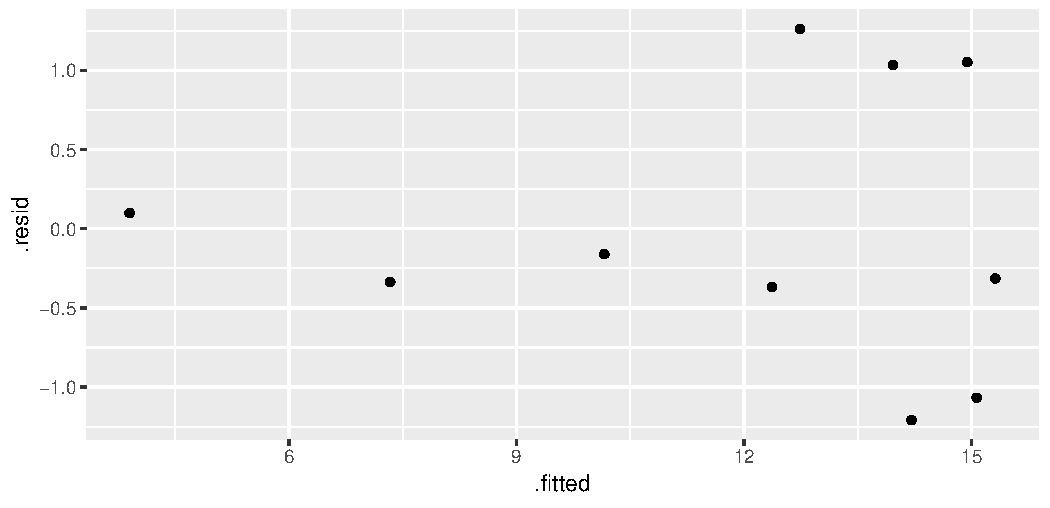
\includegraphics[width=\maxwidth]{figure/unnamed-chunk-23-1} 

\end{knitrout}

The lines are definitely \emph{not} parallel, showing that the effect
of \texttt{type} is different for medium-sized engines than for others.
  
\end{frame}

\begin{frame}[fragile]{If you don't like that\ldots}
  
  \ldots then compute the means first, in a pipe:

  \begin{small}
\begin{knitrout}
\definecolor{shadecolor}{rgb}{0.969, 0.969, 0.969}\color{fgcolor}\begin{kframe}
\begin{alltt}
\hlstd{autonoise} \hlopt \hlkwd{group_by}\hlstd{(size,type)} \hlopt
  \hlkwd{summarize}\hlstd{(}\hlkwc{mean_noise}\hlstd{=}\hlkwd{mean}\hlstd{(noise))} \hlopt
  \hlkwd{ggplot}\hlstd{(}\hlkwd{aes}\hlstd{(}\hlkwc{x}\hlstd{=size,}\hlkwc{y}\hlstd{=mean_noise,}\hlkwc{group}\hlstd{=type,}\hlkwc{colour}\hlstd{=type))}\hlopt{+}
    \hlkwd{geom_point}\hlstd{()}\hlopt{+}\hlkwd{geom_line}\hlstd{()}
\end{alltt}
\end{kframe}
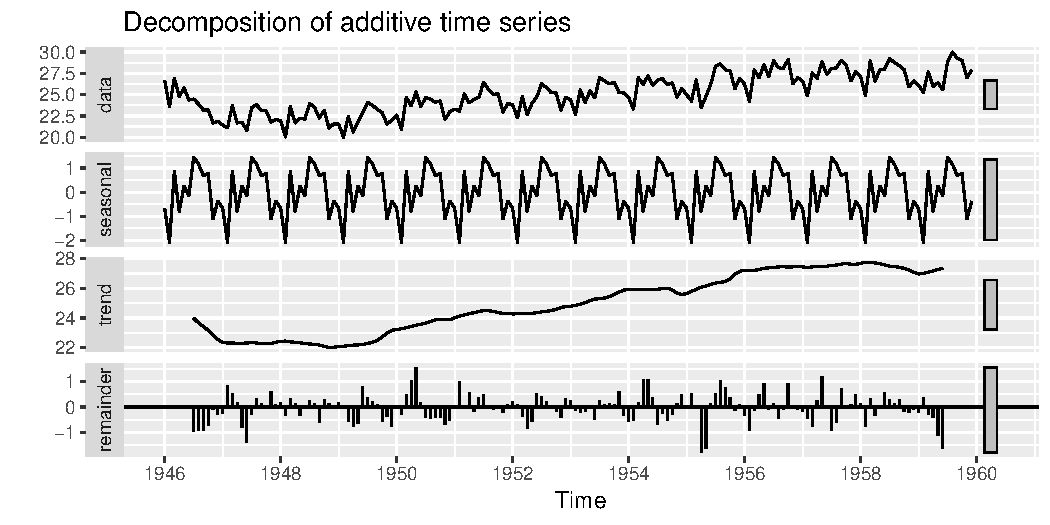
\includegraphics[width=\maxwidth]{figure/unnamed-chunk-24-1} 

\end{knitrout}
    
  \end{small}
  
\end{frame}


\begin{frame}[fragile]{Simple effects for auto noise example}
  \begin{itemize}
  \item In auto noise example, weren't interested in all comparisons
    between car size and filter type combinations.
  \item Wanted to demonstrate (lack of) difference between filter types
    \emph{for each car type}. 

  \item These are called \textbf{simple effects} of one variable
    (filter type)
    conditional on other variable (car type).

  \item To do this, pull out just the data for small cars, compare
    noise for the two filter types. Then repeat for medium and large
    cars. (Three one-way ANOVAs.)

  \end{itemize}
\end{frame}

\begin{frame}[fragile]{Do it using \texttt{dplyr} tools}
  
  \begin{itemize}
  \item Small cars:
\begin{knitrout}
\definecolor{shadecolor}{rgb}{0.969, 0.969, 0.969}\color{fgcolor}\begin{kframe}
\begin{alltt}
\hlstd{autonoise} \hlopt \hlkwd{filter}\hlstd{(size}\hlopt{==}\hlstr{"S"}\hlstd{)} \hlopt
  \hlkwd{aov}\hlstd{(noise}\hlopt{~}\hlstd{type,}\hlkwc{data}\hlstd{=.)} \hlopt \hlkwd{summary}\hlstd{()}
\end{alltt}
\begin{verbatim}
##             Df Sum Sq Mean Sq F value Pr(>F)
## type         1   33.3   33.33   0.548  0.476
## Residuals   10  608.3   60.83
\end{verbatim}
\end{kframe}
\end{knitrout}

\item No filter difference for small cars.
  

\item For Medium, change \texttt{S} to \texttt{M} and repeat.
  \end{itemize}
  
\end{frame}

\begin{frame}[fragile]{Simple effect of filter type for medium cars}
  
  {\small
\begin{knitrout}
\definecolor{shadecolor}{rgb}{0.969, 0.969, 0.969}\color{fgcolor}\begin{kframe}
\begin{alltt}
\hlstd{autonoise} \hlopt \hlkwd{filter}\hlstd{(size}\hlopt{==}\hlstr{"M"}\hlstd{)} \hlopt
  \hlkwd{aov}\hlstd{(noise}\hlopt{~}\hlstd{type,}\hlkwc{data}\hlstd{=.)} \hlopt \hlkwd{summary}\hlstd{()}
\end{alltt}
\begin{verbatim}
##             Df Sum Sq Mean Sq F value   Pr(>F)    
## type         1 1752.1  1752.1   68.93 8.49e-06 ***
## Residuals   10  254.2    25.4                     
## ---
## Signif. codes:  0 '***' 0.001 '**' 0.01 '*' 0.05 '.' 0.1 ' ' 1
\end{verbatim}
\end{kframe}
\end{knitrout}
}

\begin{itemize}
\item There \emph{is} an effect of filter type for medium cars. Look
  at means to investigate:
 
  {\footnotesize
\begin{knitrout}
\definecolor{shadecolor}{rgb}{0.969, 0.969, 0.969}\color{fgcolor}\begin{kframe}
\begin{alltt}
\hlstd{autonoise} \hlopt \hlkwd{filter}\hlstd{(size}\hlopt{==}\hlstr{"M"}\hlstd{)} \hlopt
  \hlkwd{group_by}\hlstd{(type)} \hlopt \hlkwd{summarize}\hlstd{(}\hlkwc{m}\hlstd{=}\hlkwd{mean}\hlstd{(noise))}
\end{alltt}
\begin{verbatim}
## # A tibble: 2 × 2
##     type        m
##   <fctr>    <dbl>
## 1  Octel 821.6667
## 2    Std 845.8333
\end{verbatim}
\end{kframe}
\end{knitrout}
}


  
\end{itemize}

\end{frame}


\begin{frame}[fragile]{Medium and large cars}
  
  \begin{itemize}
\item Octel filters produce \emph{less} noise for medium cars.
\item Large cars:
\begin{knitrout}
\definecolor{shadecolor}{rgb}{0.969, 0.969, 0.969}\color{fgcolor}\begin{kframe}
\begin{alltt}
\hlstd{autonoise} \hlopt \hlkwd{filter}\hlstd{(size}\hlopt{==}\hlstr{"L"}\hlstd{)} \hlopt
  \hlkwd{aov}\hlstd{(noise}\hlopt{~}\hlstd{type,}\hlkwc{data}\hlstd{=.)} \hlopt \hlkwd{summary}\hlstd{()}
\end{alltt}
\begin{verbatim}
##             Df Sum Sq Mean Sq F value Pr(>F)
## type         1     75      75   0.682  0.428
## Residuals   10   1100     110
\end{verbatim}
\end{kframe}
\end{knitrout}

\item No significant difference again.

  \end{itemize}


\end{frame}

\begin{frame}[fragile]{Simultaneous tests}
  
  \begin{itemize}
  \item When testing simple effects, doing several tests at once. (In
    this case, 3.)
  \item Have to adjust P-values for this. Eg.\ Holm:
\begin{knitrout}
\definecolor{shadecolor}{rgb}{0.969, 0.969, 0.969}\color{fgcolor}\begin{kframe}
\begin{alltt}
\hlstd{p.values}\hlkwb{=}\hlkwd{c}\hlstd{(}\hlnum{8.49e-6}\hlstd{,}\hlnum{0.428}\hlstd{,}\hlnum{0.476}\hlstd{)}
\hlstd{p.values[}\hlnum{1}\hlstd{]}\hlopt{*}\hlnum{3} \hlstd{; p.values[}\hlnum{2}\hlstd{]}\hlopt{*}\hlnum{2} \hlstd{; p.values[}\hlnum{3}\hlstd{]}\hlopt{*}\hlnum{1}
\end{alltt}
\begin{verbatim}
## [1] 2.547e-05
## [1] 0.856
## [1] 0.476
\end{verbatim}
\end{kframe}
\end{knitrout}
\item No change in rejection decisions.
\item Octel filters are significantly better in terms of noise for
  medium-sized cars, and not significantly different for other car
  sizes.
\item In no case are Octel filters significantly worse than standard
  ones. 
  \end{itemize}
  
\end{frame}

\begin{frame}[fragile]{Confidence intervals}
  
  \begin{itemize}
  \item Perhaps better way of assessing simple effects: look at
    \emph{confidence intervals} rather than tests.
  \item Gives us sense of accuracy of estimation, and thus whether
    non-significance might be lack of power: ``absence of evidence is
    not evidence of absence''.
  \item Works here because \emph{two} filter types, using
    \texttt{t.test} for each engine type.
  \item Want to show that the Octel filter is equivalent to or better
    than the standard filter, in terms of engine noise.
  \end{itemize}
  
\end{frame}

\begin{frame}[fragile]{Equivalence and noninferiority}
  
  \begin{itemize}
  \item Known as ``equivalence testing'' in medical world. A good
    read:
    \url{http://www.ncbi.nlm.nih.gov/pmc/articles/PMC3019319/}. Basic
    idea: decide on size of difference $\delta$ that would be considered
    ``equivalent'', and if CI entirely inside $\pm \delta$, have
    evidence in favour of equivalence.
  \item We really want to show that the Octel filters are ``no worse''
    than the standard one: that is, equivalent \emph{or better} than
    standard filters.
  \item Such a ``noninferiority test'' done by checking that
    \texttt{upper limit} of CI, new minus old, is \emph{less} than
    $\delta$. (This requires careful thinking about (i) which way
    around the difference is and (ii) whether a higher or lower value
    is better.)
  \end{itemize}
  
\end{frame}


\begin{frame}[fragile]{CI for small cars}
  
Same idea as for simple effect test:

\begin{knitrout}
\definecolor{shadecolor}{rgb}{0.969, 0.969, 0.969}\color{fgcolor}\begin{kframe}
\begin{alltt}
\hlstd{autonoise} \hlopt \hlkwd{filter}\hlstd{(size}\hlopt{==}\hlstr{"S"}\hlstd{)} \hlopt
  \hlkwd{t.test}\hlstd{(noise}\hlopt{~}\hlstd{type,}\hlkwc{data}\hlstd{=.)} \hlopt \hlstd{.[[}\hlstr{"conf.int"}\hlstd{]]}
\end{alltt}
\begin{verbatim}
## [1] -14.517462   7.850795
## attr(,"conf.level")
## [1] 0.95
\end{verbatim}
\end{kframe}
\end{knitrout}

  
\end{frame}
 
  

\begin{frame}[fragile]{CI for medium cars}
  

\begin{knitrout}
\definecolor{shadecolor}{rgb}{0.969, 0.969, 0.969}\color{fgcolor}\begin{kframe}
\begin{alltt}
\hlstd{autonoise} \hlopt \hlkwd{filter}\hlstd{(size}\hlopt{==}\hlstr{"M"}\hlstd{)} \hlopt
  \hlkwd{t.test}\hlstd{(noise}\hlopt{~}\hlstd{type,}\hlkwc{data}\hlstd{=.)} \hlopt \hlstd{.[[}\hlstr{"conf.int"}\hlstd{]]}
\end{alltt}
\begin{verbatim}
## [1] -30.75784 -17.57549
## attr(,"conf.level")
## [1] 0.95
\end{verbatim}
\end{kframe}
\end{knitrout}
  
\end{frame}
\begin{frame}[fragile]{CI for large cars}
  

\begin{knitrout}
\definecolor{shadecolor}{rgb}{0.969, 0.969, 0.969}\color{fgcolor}\begin{kframe}
\begin{alltt}
\hlstd{autonoise} \hlopt \hlkwd{filter}\hlstd{(size}\hlopt{==}\hlstr{"L"}\hlstd{)} \hlopt
  \hlkwd{t.test}\hlstd{(noise}\hlopt{~}\hlstd{type,}\hlkwc{data}\hlstd{=.)} \hlopt \hlstd{.[[}\hlstr{"conf.int"}\hlstd{]]}
\end{alltt}
\begin{verbatim}
## [1] -19.270673   9.270673
## attr(,"conf.level")
## [1] 0.95
\end{verbatim}
\end{kframe}
\end{knitrout}
  
\end{frame}

\begin{frame}[fragile]{CIs and noninferiority test}
  
  \begin{itemize}
  \item Suppose we decide that a 20 dB difference would be considered
    equivalent. (I have no idea whether that is reasonable.)
    
  \item Intervals: \vspace{2ex}
    
    \begin{tabular}{lrr}
      Engine size & Lower & Upper \\
      \hline
      Small & --14.5 &7.9 \\
      Medium & --30.8 &--17.6\\
      Large & --19.3&9.3\\
      \hline
    \end{tabular} \vspace{2ex}

  \item In all cases, upper limit of CI is less than 20 dB. The Octel
    filters are ``noninferior'' to the standard ones.
  \item Caution: we did 3 procedures at once again. The true
    confidence level is not 95\%. (Won't worry about that here.)
  \end{itemize}
  
\end{frame}

\begin{frame}[fragile]{Contrasts in ANOVA}
  
  \begin{itemize}
  \item Sometimes, don't want to compare \emph{all} groups, only
    \texttt{some} of them.
  \item Might be able to specify these comparisons ahead of time;
    other comparisons of no interest.
  \item Wasteful to do ANOVA and Tukey.
  \end{itemize}
  
\end{frame}

\begin{frame}[fragile]{Example: chainsaw kickback}
  
  \begin{itemize}
    \item From \url{http://www.ohio.edu/plantbio/staff/mccarthy/quantmet/lectures/ANOVA2.pdf}.
  \item Forest manager concerned about safety of chainsaws issued to
    field crew. 4 models of chainsaws, measure ``kickback'' (degrees
    of deflection) for 5 of each:
    
\begin{verbatim}
 A  B  C  D
-----------
42 28 57 29
17 50 45 29
24 44 48 22
39 32 41 34
43 61 54 30
\end{verbatim}
    
    \item So far, standard 1-way ANOVA: what differences are there
      among models?
  \end{itemize}
  
\end{frame}

\begin{frame}[fragile]{chainsaw kickback (2)}
  
  \begin{itemize}
    \item But: models A and D are designed to be used at home, while
      models B and C are industrial models.
    \item Suggests these comparisons of interest:
      \begin{itemize}
      \item home vs.\ industrial
      \item the two home models A vs.\ D
      \item the two industrial models B vs.\ C.
      \end{itemize}
    \item Don't need to compare \emph{all} the pairs of models.

  \end{itemize}
  
\end{frame}

\begin{frame}[fragile]{What is a contrast?}
  
  \begin{itemize}
  \item Contrast is a linear combination of group means.

  \item Notation: $\mu_A$ for (population) mean of group $A$, and so on.
  \item In example, compare two home models: $H_0: \mu_A-\mu_D=0$.
  \item Compare two industrial models: $H_0: \mu_B-\mu_C=0$.
  \item Compare average of two home models vs.\ average of two
    industrial models: $H_0: {1\over2}(\mu_A+\mu_D)-{1\over
      2}(\mu_B+\mu_C)=0$ or $H_0: 0.5\mu_A-0.5\mu_B-0.5\mu_C+0.5\mu_D=0$.
  \item Note that coefficients of contrasts add to 0, and right-hand
    side is 0.
  \end{itemize}
  
\end{frame}

\begin{frame}[fragile]{Contrasts in R}
  
  \begin{itemize}
  \item Comparing two home models A and D ($\mu_A-\mu_D=0$):
\begin{knitrout}
\definecolor{shadecolor}{rgb}{0.969, 0.969, 0.969}\color{fgcolor}\begin{kframe}
\begin{alltt}
\hlstd{c.home}\hlkwb{=}\hlkwd{c}\hlstd{(}\hlnum{1}\hlstd{,}\hlnum{0}\hlstd{,}\hlnum{0}\hlstd{,}\hlopt{-}\hlnum{1}\hlstd{)}
\end{alltt}
\end{kframe}
\end{knitrout}

\item Comparing two industrial models B and C ($\mu_B-\mu_C=0$):
  
\begin{knitrout}
\definecolor{shadecolor}{rgb}{0.969, 0.969, 0.969}\color{fgcolor}\begin{kframe}
\begin{alltt}
\hlstd{c.industrial}\hlkwb{=}\hlkwd{c}\hlstd{(}\hlnum{0}\hlstd{,}\hlnum{1}\hlstd{,}\hlopt{-}\hlnum{1}\hlstd{,}\hlnum{0}\hlstd{)}
\end{alltt}
\end{kframe}
\end{knitrout}

\item Comparing home average vs.\ industrial average ($0.5\mu_A-0.5\mu_B-0.5\mu_C+0.5\mu_D=0$):
  
\begin{knitrout}
\definecolor{shadecolor}{rgb}{0.969, 0.969, 0.969}\color{fgcolor}\begin{kframe}
\begin{alltt}
\hlstd{c.home.ind}\hlkwb{=}\hlkwd{c}\hlstd{(}\hlnum{0.5}\hlstd{,}\hlopt{-}\hlnum{0.5}\hlstd{,}\hlopt{-}\hlnum{0.5}\hlstd{,}\hlnum{0.5}\hlstd{)}
\end{alltt}
\end{kframe}
\end{knitrout}
  \end{itemize}
  
\end{frame}

\begin{frame}[fragile]{Orthogonal contrasts}
  
  \begin{itemize}
  \item What happens if we multiply the contrast coefficients one by one?
\begin{knitrout}
\definecolor{shadecolor}{rgb}{0.969, 0.969, 0.969}\color{fgcolor}\begin{kframe}
\begin{alltt}
\hlstd{c.home}\hlopt{*}\hlstd{c.industrial}
\end{alltt}
\begin{verbatim}
## [1] 0 0 0 0
\end{verbatim}
\begin{alltt}
\hlstd{c.home}\hlopt{*}\hlstd{c.home.ind}
\end{alltt}
\begin{verbatim}
## [1]  0.5  0.0  0.0 -0.5
\end{verbatim}
\begin{alltt}
\hlstd{c.industrial}\hlopt{*}\hlstd{c.home.ind}
\end{alltt}
\begin{verbatim}
## [1]  0.0 -0.5  0.5  0.0
\end{verbatim}
\end{kframe}
\end{knitrout}
\item in each case, the results \textbf{add up to zero}. Such
  contrasts are called \textbf{orthogonal}.

  \end{itemize}
  
\end{frame}

\begin{frame}[fragile]{Orthogonal contrasts (2)}
  
  \begin{itemize}
\item Compare these:
\begin{knitrout}
\definecolor{shadecolor}{rgb}{0.969, 0.969, 0.969}\color{fgcolor}\begin{kframe}
\begin{alltt}
\hlstd{c1}\hlkwb{=}\hlkwd{c}\hlstd{(}\hlnum{1}\hlstd{,}\hlopt{-}\hlnum{1}\hlstd{,}\hlnum{0}\hlstd{)}
\hlstd{c1}
\end{alltt}
\begin{verbatim}
## [1]  1 -1  0
\end{verbatim}
\begin{alltt}
\hlstd{c2}\hlkwb{=}\hlkwd{c}\hlstd{(}\hlnum{0}\hlstd{,}\hlnum{1}\hlstd{,}\hlopt{-}\hlnum{1}\hlstd{)}
\hlstd{c2}
\end{alltt}
\begin{verbatim}
## [1]  0  1 -1
\end{verbatim}
\begin{alltt}
\hlstd{c1}\hlopt{*}\hlstd{c2}
\end{alltt}
\begin{verbatim}
## [1]  0 -1  0
\end{verbatim}
\end{kframe}
\end{knitrout}
Does not add up to zero, so \texttt{c1} and \texttt{c2} are \emph{not}
orthogonal.
\item Orthogonal contrasts are much easier to deal with. 

\item Can use non-orthogonal contrasts, but much more trouble (and
  beyond us).
  \end{itemize}
\end{frame}


\begin{frame}[fragile]{Starting the analysis}
  
\begin{knitrout}
\definecolor{shadecolor}{rgb}{0.969, 0.969, 0.969}\color{fgcolor}\begin{kframe}
\begin{alltt}
\hlstd{chain.wide}\hlkwb{=}\hlkwd{read.table}\hlstd{(}\hlstr{"chainsaw.txt"}\hlstd{,}\hlkwc{header}\hlstd{=T)}
\hlstd{chain.wide}
\end{alltt}
\begin{verbatim}
##    A  B  C  D
## 1 42 28 57 29
## 2 17 50 45 29
## 3 24 44 48 22
## 4 39 32 41 34
## 5 43 61 54 30
\end{verbatim}
\end{kframe}
\end{knitrout}

Need all the kickbacks in \emph{one} column:

\begin{knitrout}
\definecolor{shadecolor}{rgb}{0.969, 0.969, 0.969}\color{fgcolor}\begin{kframe}
\begin{alltt}
\hlkwd{library}\hlstd{(tidyr)}
\hlstd{chain}\hlkwb{=}\hlkwd{gather}\hlstd{(chain.wide,model,kickback,A}\hlopt{:}\hlstd{D,}
  \hlkwc{factor_key}\hlstd{=T)}
\end{alltt}
\end{kframe}
\end{knitrout}
  
\end{frame}

\begin{frame}[fragile]{Starting the analysis (2)}
  
  The proper data frame:
  
  \begin{multicols}{2}
\begin{knitrout}
\definecolor{shadecolor}{rgb}{0.969, 0.969, 0.969}\color{fgcolor}\begin{kframe}
\begin{alltt}
\hlstd{chain[}\hlnum{1}\hlopt{:}\hlnum{10}\hlstd{,]}
\end{alltt}
\begin{verbatim}
##    model kickback
## 1      A       42
## 2      A       17
## 3      A       24
## 4      A       39
## 5      A       43
## 6      B       28
## 7      B       50
## 8      B       44
## 9      B       32
## 10     B       61
\end{verbatim}
\end{kframe}
\end{knitrout}

\begin{knitrout}
\definecolor{shadecolor}{rgb}{0.969, 0.969, 0.969}\color{fgcolor}\begin{kframe}
\begin{alltt}
\hlstd{chain[}\hlnum{11}\hlopt{:}\hlnum{20}\hlstd{,]}
\end{alltt}
\begin{verbatim}
##    model kickback
## 11     C       57
## 12     C       45
## 13     C       48
## 14     C       41
## 15     C       54
## 16     D       29
## 17     D       29
## 18     D       22
## 19     D       34
## 20     D       30
\end{verbatim}
\end{kframe}
\end{knitrout}
  \end{multicols}
\end{frame}

\begin{frame}[fragile]{Setting up contrasts}
  
\begin{knitrout}
\definecolor{shadecolor}{rgb}{0.969, 0.969, 0.969}\color{fgcolor}\begin{kframe}
\begin{alltt}
\hlkwd{attach}\hlstd{(chain)}
\hlstd{m}\hlkwb{=}\hlkwd{cbind}\hlstd{(c.home,c.industrial,c.home.ind)}
\hlstd{m}
\end{alltt}
\begin{verbatim}
##      c.home c.industrial c.home.ind
## [1,]      1            0        0.5
## [2,]      0            1       -0.5
## [3,]      0           -1       -0.5
## [4,]     -1            0        0.5
\end{verbatim}
\begin{alltt}
\hlkwd{contrasts}\hlstd{(model)}\hlkwb{=}\hlstd{m}
\end{alltt}
\end{kframe}
\end{knitrout}

  
\end{frame}

\begin{frame}[fragile]{ANOVA as regression}

  Now run ANOVA \emph{as if regression}:

  {\scriptsize
\begin{knitrout}
\definecolor{shadecolor}{rgb}{0.969, 0.969, 0.969}\color{fgcolor}\begin{kframe}
\begin{alltt}
\hlstd{chain.1}\hlkwb{=}\hlkwd{lm}\hlstd{(kickback}\hlopt{~}\hlstd{model)}
\hlkwd{summary}\hlstd{(chain.1)}
\end{alltt}
\begin{verbatim}
## 
## Call:
## lm(formula = kickback ~ model)
## 
## Residuals:
##    Min     1Q Median     3Q    Max 
## -16.00  -7.10   0.60   6.25  18.00 
## 
## Coefficients:
##                   Estimate Std. Error t value Pr(>|t|)    
## (Intercept)         38.450      2.179  17.649 6.52e-12 ***
## modelc.home          2.100      3.081   0.682  0.50524    
## modelc.industrial   -3.000      3.081  -0.974  0.34469    
## modelc.home.ind    -15.100      4.357  -3.466  0.00319 ** 
## ---
## Signif. codes:  0 '***' 0.001 '**' 0.01 '*' 0.05 '.' 0.1 ' ' 1
## 
## Residual standard error: 9.743 on 16 degrees of freedom
## Multiple R-squared:  0.4562,	Adjusted R-squared:  0.3542 
## F-statistic: 4.474 on 3 and 16 DF,  p-value: 0.01833
\end{verbatim}
\end{kframe}
\end{knitrout}
}

\end{frame}

\begin{frame}[fragile]{Conclusions}
  
  \begin{itemize}
  \item Two home models not sig.\ diff.\ (P-value 0.51)
  \item Two industrial models not sig.\ diff.\ (P-value 0.34)
  \item Home, industrial
    models \emph{are} sig.\ diff.\ (P-value 0.0032).
  \item Means by model:
\begin{knitrout}
\definecolor{shadecolor}{rgb}{0.969, 0.969, 0.969}\color{fgcolor}\begin{kframe}
\begin{alltt}
\hlkwd{aggregate}\hlstd{(kickback}\hlopt{~}\hlstd{model,chain,mean)}
\end{alltt}
\begin{verbatim}
##   model kickback
## 1     A     33.0
## 2     B     43.0
## 3     C     49.0
## 4     D     28.8
\end{verbatim}
\end{kframe}
\end{knitrout}
\item Home models have less kickback than industrial ones.
\item Makes sense because industrial users should get training to cope
  with additional kickback.
  \end{itemize}
  
\end{frame}

